
In the first section of this chapter, we saw why abstracting access to container elements with iterators is key for building general-purpose algorithms. However, it should be useful for you to practice writing such an algorithm because it can help you better understand the use of iterators. Therefore, in this section, we will write a general-purpose algorithm.

The standard library features many such algorithms. One that is missing is a zipping algorithm. What zipping means is actually interpreted or understood differently by different people. For some, zipping means taking two or more input ranges and creating a new range with the elements from the input ranges intercalated. This is exemplified in the following diagram:

\begin{center}
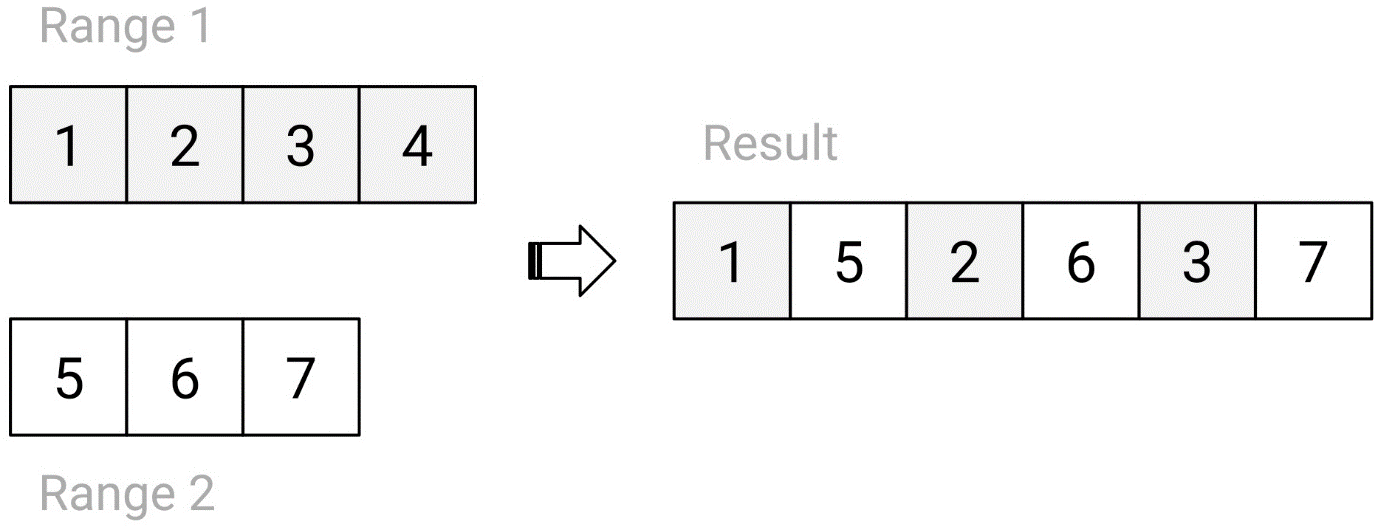
\includegraphics[width=0.6\textwidth]{content/3/chapter8/images/4.png}\\
Figure 8.4
\end{center}

For others, zipping means taking two or more input ranges and creating a new range, with elements being tuples formed from the elements of the input ranges. This is shown in the next diagram:

\begin{center}
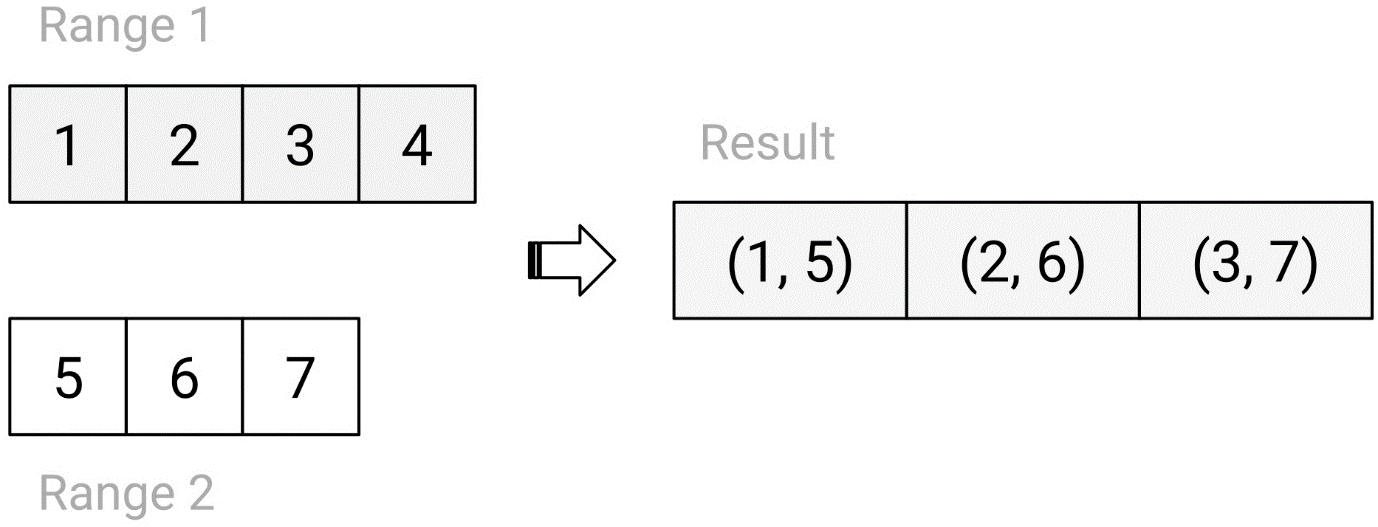
\includegraphics[width=0.6\textwidth]{content/3/chapter8/images/5.png}\\
Figure 8.5
\end{center}

In this section, we will implement the first algorithm. In order to avoid confusion, we will call this flatzip. Here are the requirements for it:

\begin{itemize}
\item
The algorithm takes two input ranges and writes to an output range.

\item
The algorithm takes iterators as arguments. A pair of first and last input iterators define the bounds of each input range. An output iterator defines the beginning of the output range where the elements will be written to.

\item
The two input ranges should contain elements of the same type. The output range must have elements of the same type or a type to which the input type is implicitly convertible.

\item
If the two input ranges are of different sizes, the algorithm stops when the smallest of the two has been processed (as shown in the previous diagrams).

\item
The return value is the output iterator to the one-past-the-last element that was copied.
\end{itemize}

A possible implementation for the described algorithm is shown in the following listing:

\begin{lstlisting}[style=styleCXX]
template <typename InputIt1, typename InputIt2,
		  typename OutputIt>
OutputIt flatzip(
	InputIt1 first1, InputIt1 last1,
	InputIt2 first2, InputIt2 last2,
	OutputIt dest)
{
	auto it1 = first1;
	auto it2 = first2;
	
	while (it1 != last1 && it2 != last2)
	{
		*dest++ = *it1++;
		*dest++ = *it2++;
	}

	return dest;
}
\end{lstlisting}

As you can see in the snippet, the implementation is quite simple. All we do here is iterate through both input ranges at the same time and copy elements alternately from them to the destination range. The iteration on both input ranges stops when the end of the smallest range is reached. We can use this algorithm as follows:

\begin{lstlisting}[style=styleCXX]
// one range is empty
std::vector<int> v1 {1,2,3};
std::vector<int> v2;
std::vector<int> v3;

flatzip(v1.begin(), v1.end(), v2.begin(), v2.end(),
		std::back_inserter(v3));
assert(v3.empty());

// neither range is empty
std::vector<int> v1 {1, 2, 3};
std::vector<int> v2 {4, 5};
std::vector<int> v3;

flatzip(v1.begin(), v1.end(), v2.begin(), v2.end(),
		std::back_inserter(v3));
assert(v3 == std::vector<int>({ 1, 4, 2, 5 }));
\end{lstlisting}

These examples use std::vector for both the input and output ranges. However, the flatzip algorithm knows nothing about containers. The elements of the container are accessed with the help of iterators. Therefore, as long as the iterators meet the specified requirements, we can use any container. This includes the circular\_buffer container we previously wrote since circular\_buffer\_container meets the requirements for both the input and output iterator categories. This means we can also write the following snippet:

\begin{lstlisting}[style=styleCXX]
circular_buffer<int, 4> a({1, 2, 3, 4});
circular_buffer<int, 3> b({5, 6, 7});
circular_buffer<int, 8> c(0);

flatzip(a.begin(), a.end(), b.begin(), b.end(), c.begin());

std::vector<int> v;
for (auto e : c)
	v.push_back(e);
assert(v == std::vector<int>({ 1, 5, 2, 6, 3, 7, 0, 0 }));
\end{lstlisting}

We have two input circular buffers: a, which has four elements, and b, which has three elements. The destination circular buffer has a capacity of eight elements, all initialized with zero. After applying the flatzip algorithm, six elements of the destination circular buffer will be written with values from the a and b buffers. The result is that the circular buffer will contain the elements 1, 5, 2, 6, 3, 7, 0, 0.













